% !TeX root = main.tex

\hypertarget{quadratic-functions}{%
\section{Quadratic Functions}\label{quadratic-functions}}

\hypertarget{maximize-the-revenue}{%
\subsection{Maximize the Revenue}\label{maximize-the-revenue}}

When price increases, demand decreases and vice verse. A retail store
found that the price \(p\) as a function of the demand \(x\) for a
certain product is \(p(x)=100-\frac12 x\). The revenue \(R\) of selling
\(x\) units is \(R=x\cdot p(x)=x(100-\frac12x)\). To maximize the
revenue, what should be the price?

\hypertarget{the-graph-of-a-quadratic-function}{%
\subsection{The Graph of a Quadratic
Function}\label{the-graph-of-a-quadratic-function}}

The graph of a quadratic function \(f(x)=ax^2+bx+c\), \(a\neq 0\), is
called a \textbf{\emph{parabola}}.

By completing the square, a quadratic function \(f(x)=ax^2+bx+c\) can
always be written in the form \(f(x)=a(x-h)^2+k\), where
\(h=-\dfrac{b}{2a}\) and \(k=f(h)=f\left(-\dfrac{b}{2a}\right)\).

\begin{enumerate}[sepno]
\item
  The line \(x=h=-\dfrac{b}{2a}\) is called the \textbf{\emph{axis of
  symmetry}} of the parabola.
\item
  The point
  \((h, k)=\left(-\dfrac{b}{2a}, f\left(-\dfrac{b}{2a}\right)\right)\)
  is called the \textbf{\emph{vertex}} of the parabola.
\end{enumerate}

\hypertarget{the-minimum-or-maximum-of-a-quadratic-function}{%
\subsection{The Minimum or Maximum of a Quadratic
Function}\label{the-minimum-or-maximum-of-a-quadratic-function}}

Consider the quadratic function \(f(x)=ax^2+bx+c\), \(a\neq 0\).

\begin{enumerate}[sepno]
\item
  If \(a>0\), then the parabola opens upward and \(f\) has a minimum
  \(f\left(-\dfrac{b}{2a}\right)\) at the vertex.
\item
  If \(a<0\), then the parabola opens downward and \(f\) has a maximum
  \(f\left(-\dfrac{b}{2a}\right)\) at the vertex.
\end{enumerate}

\hypertarget{intercepts-of-a-quadratic-function}{%
\subsection{Intercepts of a Quadratic
Function}\label{intercepts-of-a-quadratic-function}}

Consider the quadratic function \(f(x)=ax^2+bx+c\), \(a\neq 0\).

\begin{enumerate}[sepno]
\item
  The \(y\)-intercept is \((0, f(0))=(0, c)\).
\item
  The \(x\)-intercepts, if exist, are the solutions of the equation
  \(ax^2+bx+c=0\).
\end{enumerate}

\begin{example}

Does the function \(f(x)=2x^2-4x-6\) have a maximum or minimum? Find it.

\end{example}
\vspace*{6\baselineskip}

\begin{example}

Consider the function \(f(x)=-x^2+3x+6\). Find values of \(x\) such that
\(f(x)=2\).

\end{example}
\vspace*{6\baselineskip}

\begin{example}

A quadratic function \(f\) whose the vertex is \((1, 2)\) has a
\(y\)-intercept \((0, -3)\). Find the equation that defines the
function.

\end{example}
\vspace*{6\baselineskip}

\subsection{Practice}

\begin{exercise}

Sketch the graph of the quadratic functions \(f(x)=-(x-2)^2+4\) and find

\begin{enumerate}
\item
  the coordinates of the \(x\)-intercepts,
\item
  the coordinates of the \(y\)-intercept,
\item
  the equation of the axis of symmetry,
\item
  the coordinates of the vertex.
\item
  the interval of \(x\) values such that \(f(x)\geq 0\).
\end{enumerate}

\end{exercise}

\begin{exercise}

Sketch the graph of the quadratic functions \(f(x)=x^2+2x-3\) and find

\begin{enumerate}
\item
  the coordinates of the \(x\)-intercepts,
\item
  the coordinates of the \(y\)-intercept,
\item
  the equation of the axis of symmetry,
\item
  the coordinates of the vertex.
\item
  the interval of \(x\) values such that \(f(x)>0\).
\end{enumerate}

\end{exercise}

\begin{exercise}

Consider the parabola in the graph.

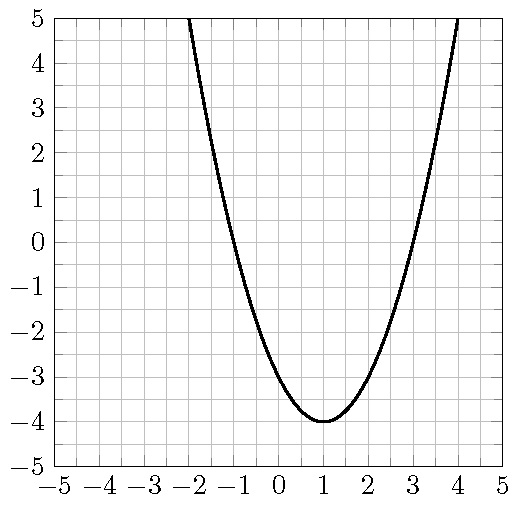
\includegraphics{figs/tikz-exercise-graph-quadratic-1.png}

\begin{enumerate}
\item
  Determine the coordinates of the \(x\)-intercepts.
\item
  Determine the coordinates of the \(y\)-intercept.
\item
  Determine the coordinates of the vertex.
\item
  For what values of \(x\) is \(f(x)=-3\).
\item
  Find an equation for the function.
\end{enumerate}

\end{exercise}

\begin{exercise}

Consider the parabola in the graph.

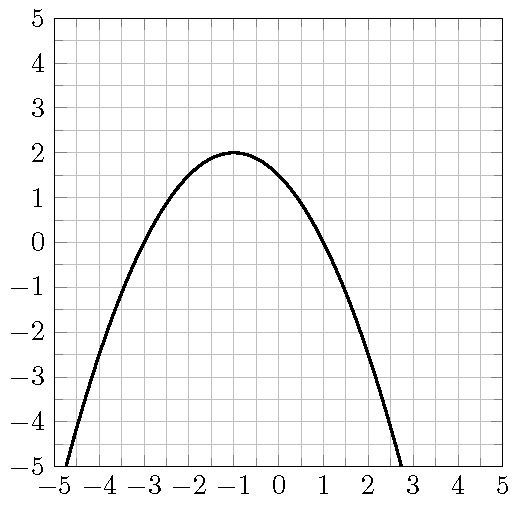
\includegraphics{figs/tikz-exercise-graph-quadratic-2.png}

\begin{enumerate}
\item
  Determine the coordinates of the \(x\)-intercepts.
\item
  Determine the coordinates of the \(y\)-intercept.
\item
  Determine the coordinates of the vertex.
\item
  For what values of \(x\) is \(f(x)=\frac{3}{2}\).
\item
  Find an equation for the function.
\end{enumerate}

\end{exercise}

\begin{exercise}

A store owner estimates that by charging \(x\) dollars each for a
certain cell phone case, he can sell \(d(x)=40 - x\) phone cases each
week. The revenue in dollars is \(R(x)=xd(x)\) when the selling price of
a cell phone case is \(x\), Find the selling price that will maximize revenue,
and then find the amount of the maximum revenue.

\end{exercise}
\vspace*{6\baselineskip}

\begin{exercise}

A ball is thrown upwards from a rooftop. It will reach a maximum
vertical height and then fall back to the ground. The height \(h(t)\) of
the ball from the ground after time \(t\) seconds is
\(h(t)=-16t^2 + 48t + 160\) feet. How long it will take the ball to hit
the ground?

\end{exercise}
\vspace*{6\baselineskip}

\begin{exercise}

A ball is thrown upward from the ground with an initial velocity \(v_0\)
ft/sec.~The height \(h(t)\) of the ball after \(t\) seconds is
\(h(t)= -16t^2 + v_0t\). The ball hits the ground after 4 seconds. Find
the maximum height and how long it will take the ball to reach the
maximum height.

\end{exercise}
\vspace*{6\baselineskip}

\begin{exercise}

A toy factory estimates that the demand of a particular toy is
\(300 -x\) units each week if the price is \$\(x\) dollars per unit.
Each week there is a fixed cost \$40,000 to produce the demanded toys.
The weekly revenue is a function of the price given by \(R(x)=x(30-x)\)

\begin{enumerate}
\item
  Find the function that models the weekly revenue, \(R\), received when
  the selling price is \$\(x\) per unit.
\item
  What the price range so the the revenue is nonnegative.
\end{enumerate}

\end{exercise}

